
\section{Performing a Maven Release}

In the last task, you will need to submit your Java code by performing a release of your code. But remember that Maven release plug-in will check if all the changes you have made have been checked into the remote repository (i.e. GitHub in our case). So, let's perform a git-commit and a git-push.

\begin{enumerate}

\begin{figure}
\hspace{-1em}
\begin{minipage}{0.5\textwidth}
\centering
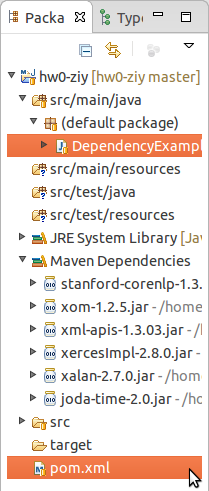
\includegraphics[scale=0.3]{simple-code-05-commit}
\caption{Performing a git-commit/push before preparing a release\label{simple-code-05-commit}}
\end{minipage}
\hfill
\begin{minipage}{0.5\textwidth}
\centering
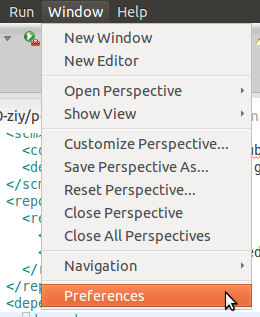
\includegraphics[scale=0.3]{submit-01-preference}
\caption{Starting to add an external Maven executable\label{submit-01-preference}}
\end{minipage}
\hspace{-1em}
\end{figure}

\item Similar to what you did earlier, you execute git-commit and git-push to the project, and you could see the ``greater than'' symbol disappears and a ``master'' label is attached to project path, which means you are successful with your git-commit and git-push.

\begin{figure}
\hspace{-2em}
\begin{minipage}{0.5\textwidth}
\centering
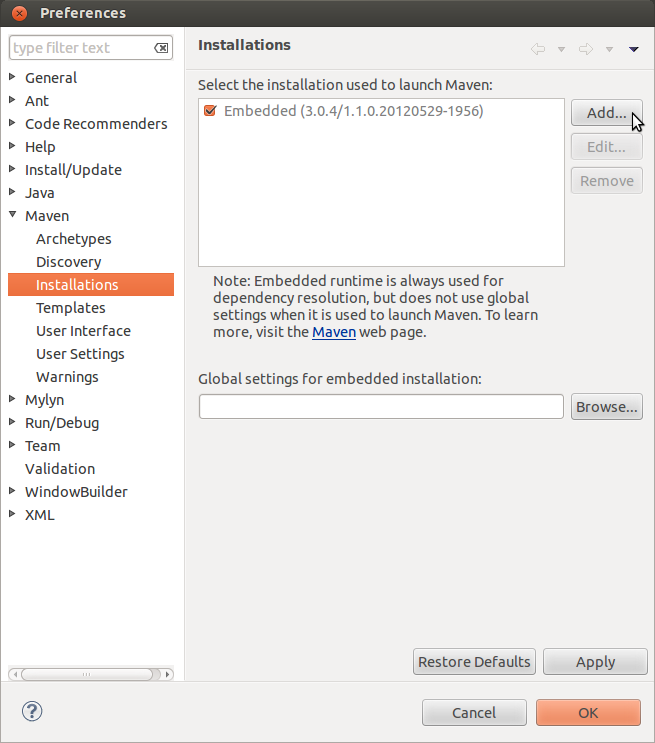
\includegraphics[scale=0.3]{submit-02-add-maven}
\caption{Adding another Maven executable\label{submit-02-add-maven}}
\end{minipage}
\hfill
\begin{minipage}{0.5\textwidth}
\centering
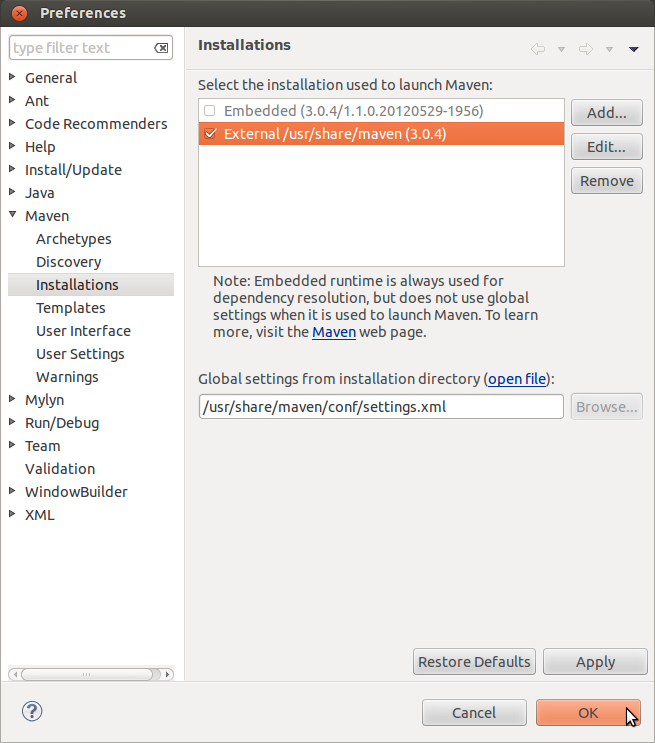
\includegraphics[scale=0.3]{submit-03-add-maven-done}
\caption{Viewing the added external Maven\label{submit-03-add-maven-done}}
\end{minipage}
\hspace{-2em}
\end{figure}

\item Sometimes, the embedded Maven runtime from m2e cannot be succesfully executed to perform a release goal. Therefore, we should add the externally installed Maven runtime into the Eclipse. Click \textbf{Window} (or \textbf{Edit}) $\rightarrow$ \textbf{Preferences} (see Figure \ref{submit-03-add-maven-done}).
\item Select \textbf{Maven} $\rightarrow$ \textbf{Installations}. You will see the ``Embedded'' runtime (as shown in Figure \ref{submit-02-add-maven}). Click \textbf{Add\ldots} to locate the installation path of your Maven runtime.
\item Then, you could see an ``External'' runtime in the installation lists. See Figure \ref{submit-03-add-maven-done}.

\begin{figure}
\centering
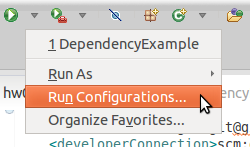
\includegraphics[scale=0.3]{submit-04-run-config}
\caption{Getting ready for a release\label{submit-04-run-config}}
\end{figure}

\item Now you can execute a Maven goal within Eclipse (of course, you can also do that outside Eclipse from command line). Click the down-arrow next to the \textbf{Run} button, and select \textbf{Run Configurations\ldots}. See Figure \ref{submit-04-run-config}.

\begin{figure}
\centering
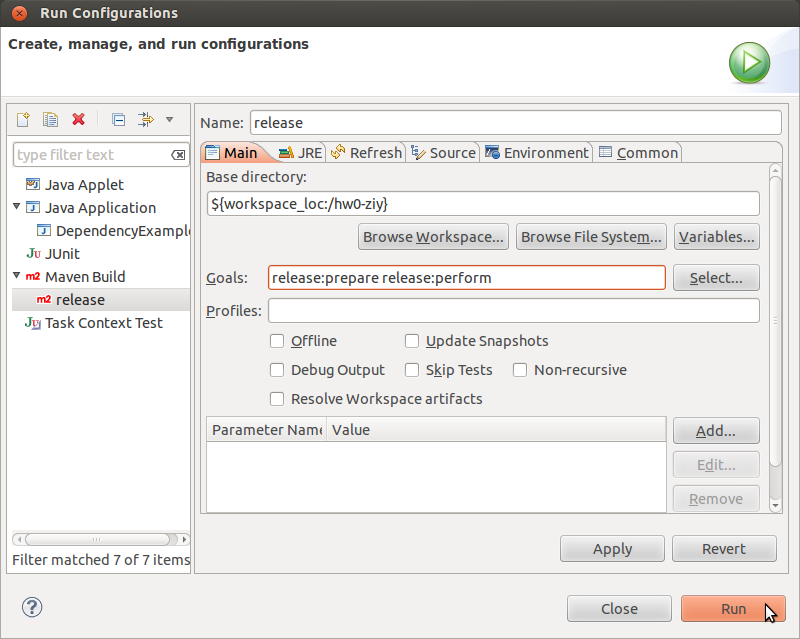
\includegraphics[scale=0.3]{submit-05-run-config-done}
\caption{Configuring Maven goal\label{submit-05-run-config-done}}
\end{figure}

\item In the ``Run Configurations'' window, double-click \textbf{Maven Build} to create a new Maven goal. See Figure \ref{submit-05-run-config-done}. Rename your run configuration name as ``release'' (optional), and click \textbf{Browse Workspace\ldots} to select your project, and type in your goals as follows:

\begin{verbatim}
release:prepare release:perform
\end{verbatim}

This actually defines two goals ``release:prepare'' and ``release:perform''. As you will probably encounter tons of errors during this step, we should review some details of the Maven release.

The Maven guide\footnote{\url{https://maven.apache.org/guides/mini/guide-releasing.html}} tells us what is happening behind these two goals:

\begin{quote}
The release:prepare goal will:

\begin{enumerate}
\item Verify that there are no uncommitted changes in the workspace.
\item Prompt the user for the desired tag, release and development version names.
\item Modify and commit release information into the pom.xml file.
\item Tag the entire project source tree with the new tag name.
\end{enumerate}

The release:perform goal will:

\begin{enumerate}
\item Extract file revisions versioned under the new tag name.
\item Execute the maven build lifecycle on the extracted instance of the project.
\item Deploy the versioned artifacts to appropriate local and remote repositories.
\end{enumerate}
\end{quote}

If the goals are not executed sucessfully, a relatively useful message will be printed out to console to help you discover where the problem is.

\begin{figure}
\centering
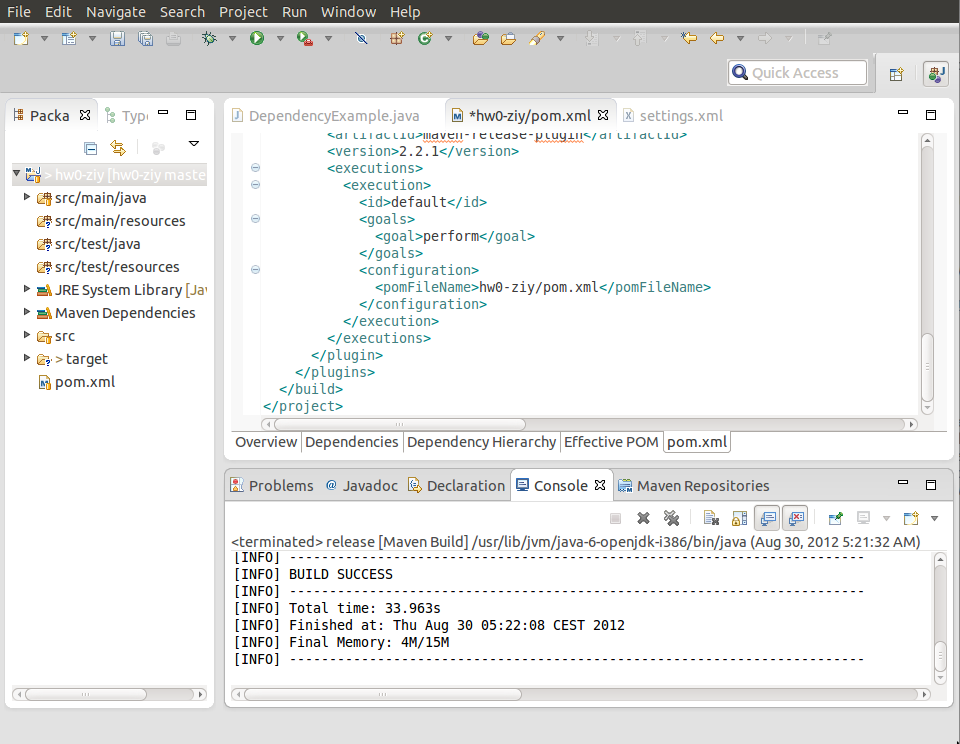
\includegraphics[scale=0.3]{submit-06-release}
\caption{A successful release!\label{submit-06-release}}
\end{figure}

\item Finally after you fixed all the problems (if any), you could see the very pleasant ``BUILD SUCCESS'' message in the console (as shown in Figure \ref{submit-06-release}), which means you've done with your Homework 0! Congratulations!

\begin{qa}
\item[Q1] The ``release:prepare'' goal could be executed successfully, but there was an error during ``release:perform''. How can I start all over again?\footnote{Reported by Kartik Mandaville.}
\item[A1] A successful ``prepare'' with an unsuccessful ``perform'' always leads to a very subtle situation. Sometimes, you can try to execute a ``release:rollback'' Maven goal to revert to the previous status, or you are try to manually delete the \verb|release.properties| file under your project diretory, and make sure you are now working on a SNAPSHOT version. (You can check your version from Maven POM Editor, and you have an opened Maven POM Editor, be sure to close it and open it again since it will not be automatically refreshed after you execute a Maven goal.) If it is no longer a SNAPSHOT version, you should modify the \textbf{Version} field to something like ``0.0.2-SNAPSHOT'' (without quotes). You might want to refer to \url{http://maven.apache.org/guides/mini/guide-releasing.html} about the details of the release process.
\item[Q2] What if I find some bugs after it has been released? How can I resubmit my code?
\item[A2] You can look at the ``Overview'' tab in the Maven POM Editor for your pom.xml file. The version should be ``0.0.2-SNAPSHOT'', which indicates a previous version has been generated. Now, you could redo this task (git-commit, git-push, run Maven goals) to release the version 0.0.2. We will evaluate your code based on the latest release.
\item[Q3] How could I check if my submission is successful?
\item[A3] First of all, don't worry about it, even if by the deadline, we haven't received your submission, we will notify you, and help you check what the problem may be before you start Homework 1.

If you want to check your submission, you can go to \url{http://mu.lti.cs.cmu.edu:8081/nexus/index.html} back again, and log in with your password, go to \textbf{View/Repositories} $\rightarrow$ \textbf{Repositories} on the left, then click \textbf{Course Releases} on the right, unfold directories along the groupId path, and if you see your artifact at the end, then you've done!
\end{qa}

\end{enumerate}